\subsection{LPCCs}
LPCCs are another type of cepstral coefficients widely used in speech processing~\cite{jahangir:review}. As mentioned in the section~\vref{sec:feature_extraction}, spectral features represent phonetic information, as they are derived directly from spectra. The features extracted from spectra, using the energy values of linearly arranged filter banks, equally emphasize the contribution of all frequency components of a speech signal. In this context, LPCCs are used to capture emotion-specific information manifested through vocal tract features~\cite{rao:spectral}.

As in the case of MFCCs, the Linear Predictive (LP) analysis requires multiple steps, exemplified in the figure \vref{fig:lpc}, that represents the steps from the speech signal to the LPCs (Linear Predictive Coefficients). The next step is to actually extract the cepstral coefficients, as shown in Figure~\vref{fig:lpcc}.
\begin{figure}
	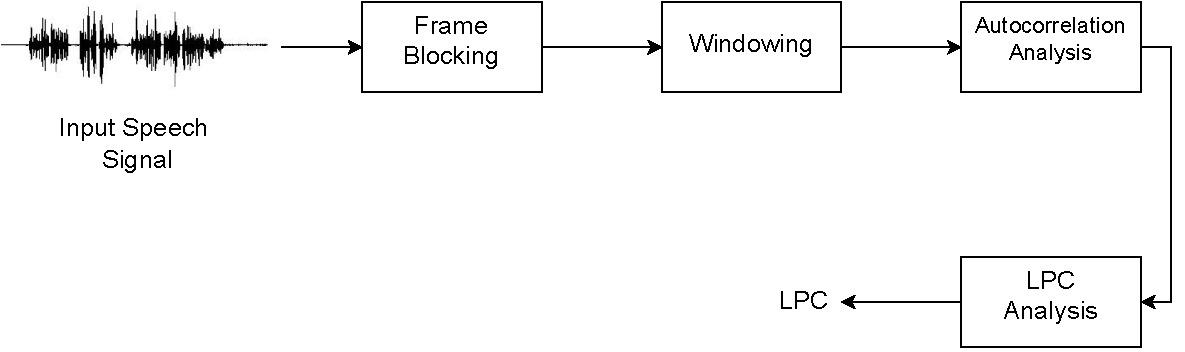
\includegraphics[width=0.5\textwidth]{images/lpc}
	\caption{LPC block diagram.}
	\label{fig:lpc}
\end{figure}
\begin{figure}
	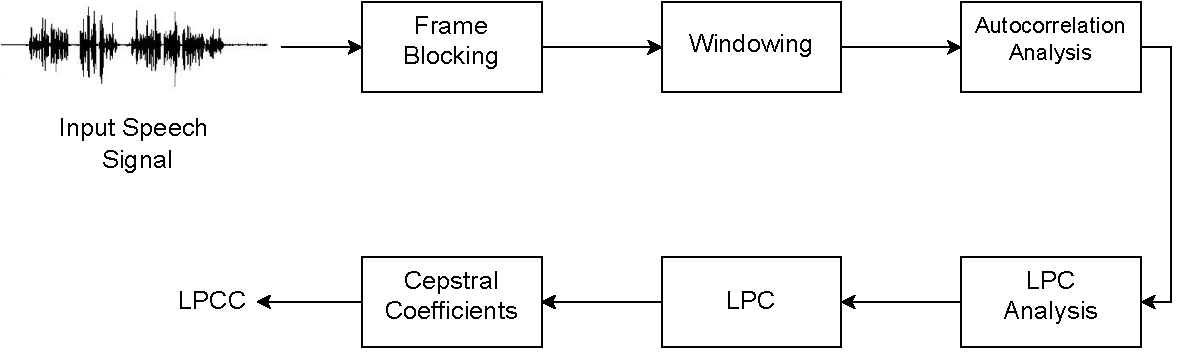
\includegraphics[width=0.5\textwidth]{images/lpcc}
	\caption{LPCC block diagram.}
	\label{fig:lpcc}
\end{figure}

In this work we extracted from the speech signal 13 LPCCs per speech frame of \SI{16}{ms}, using an overlap of \SI{8}{ms} and the \textit{hann} windowing.

\subsubsection{Cepstrum and LPCCs Calculation}

Cepstrum may be obtained using linear prediction analysis of a speech signal. The basic idea behind linear predictive analysis is that the $n$th speech sample can be
estimated by a linear combination of its previous $p$ samples as shown in the following equation~\cite{rao:spectral}:

\begin{multline}
	s(n) \thickapprox a_1s(n - 1) + a_2s(n - 2) +\\+ a_3s(n - 3) + \dots + a_ps(n - p)
\end{multline}
where $a_1, a_2, a_3, \dots$ are assumed to be constants over a speech analysis frame. These are known as predictor coefficients or linear predictive coefficients. These coefficients are used to predict the speech samples, then we can calculate the error as the difference of actual and predicted speech samples, by the following formula:

\begin{equation}
	e(n) = s(n) - \hat{s}(n) = s(n) - \sum_{k = 1}^{p}a_ks(n - k)
\end{equation}
where $e(n)$ is the error in prediction, $s(n)$ is the original speech signal, $\hat{s}(n)$ is a predicted speech signal and $a_k$s are the predictor coefficients.

To compute a unique set of predictor coefficients, the sum of squared differences between the actual and predicted speech samples has to be minimized (error minimization) as shown in the next equation~\cite{rao:spectral}:

\begin{equation}
	\min_{a_1, ..., a_p} E_n = \sum_{m} \left[ s_n(m) - \sum_{k = 1}^{p}a_k s_n (m - k)\right]^2
\end{equation}
where $m$ is the number of samples in an analysis frame. To obtain the LPCs from the equation above, $E_n$ is differentiated with respect to each $a_k$ and the result is equated to zero:

\begin{equation}
	\frac{\partial E_n}{\partial a_k} = 0, \quad \text{for} \quad k = 1, 2, 3, \dots, p
\end{equation}
After finding each $a_k$ for $k \in \{1, 2, ..., p\}$, cepstral coefficients (LPCCs) can be computed using the following recurrence relationship~\cite{rao:spectral}:

\begin{gather}
	C_0 = \log_{e}p\\	
	C_m = a_m + \sum_{k = 1}^{m - 1} \frac{k}{m} C_k a_{m - k}, \quad \text{for }  \quad 1 < m < p \quad \text{and}\\
	C_m = \sum_{k = m - p}^{m - 1} \frac{k}{m} C_k a_{m - k}, \quad \text{for} \quad m > p
\end{gather}